%% ==============================
\chapter{\iflanguage{ngerman}{Implementierung}{Implementation}}
\label{sec:implementation}
%% ==============================




Nachdem im letzten Kapitel das Softwaredesign besprochen wurde, beschäftigt sich das Kommende mit der Implementierung an sich.


Wie im Kapitel \nameref{sec:methods} schon erwähnt, wurden bei der Implementierung verschiedene Ausnahmen getroffen, um das Ergebnis und die Rechenzeit zu verbessern. Beispielsweise 


Bei der Berechnung der LH-Werte passiert es, bei ungefähr 2-\%-3\% der Fälle, dass ein Iterationsschritt außerhalb des Volumens landen würde. In diesem Fall, wird der letzte besuchte Voxel als Ergebnis für die Integration genommen. Des Weiteren kommt es bei zirka 25\% aller Berechnung dazu, dass die LH-Werte vertauscht waren, also der Low- größer als der High-Wert war. Dem wird entgegengewirkt, indem bei einem Vorkommen dieses Problems die beiden Werte vertauscht gespeichert werden. Es war noch nicht möglich den Grund für diese Verwechslung herauszufinden.

Es ergaben sich bei der Implementierung verschiedene Probleme. Beispielsweise wurde anfangs das Verfahren mit MRT-Daten getestet. Dies war von wenig Erfolg, da die Volumendaten große Unterschiede zu den CT-Daten aufweisen und somit das Verfahren nicht funktionierte.



Bei der Kalkulation der Gradienten, wird eine Gewichtung und die Koordinaten aller 64 Punkte in der lokalen Nachbarschaft benötigt. Da das gesamte Volumen die selbe Voxellänge hat und die Koordinaten in der lokalen Nachbarschaft immer gleich sind, konnten diese beiden Werte für alle 64 Nachbarn einmalig in einem Vorverarbeitungsschritt berechnet werden. Sie werden dabei in einem 64 Elemente großes Array mit der gleichen Nummerierung wie in \autoref{fig:nachbarschaft} gespeichert. Die Implementierung ist in \autoref{fig:gewicht_koord} zu sehen. Es muss bei Kalkulation jedes Gradienten lediglich die beiden Arrays durch iteriert  werden.


\begin{figure}[!h] 

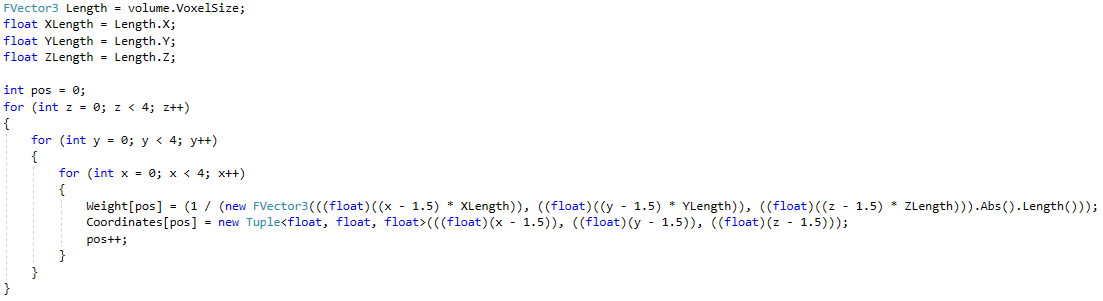
\includegraphics[width=1.2\textwidth]{Logos/Nachbar_Code_Hell_Kurz.PNG}
\caption{Implementierung der Berechnung der Gewichte und Koordinaten} 
\label{fig:gewicht_koord} 
\end{figure}



\begin{figure}[!h] 
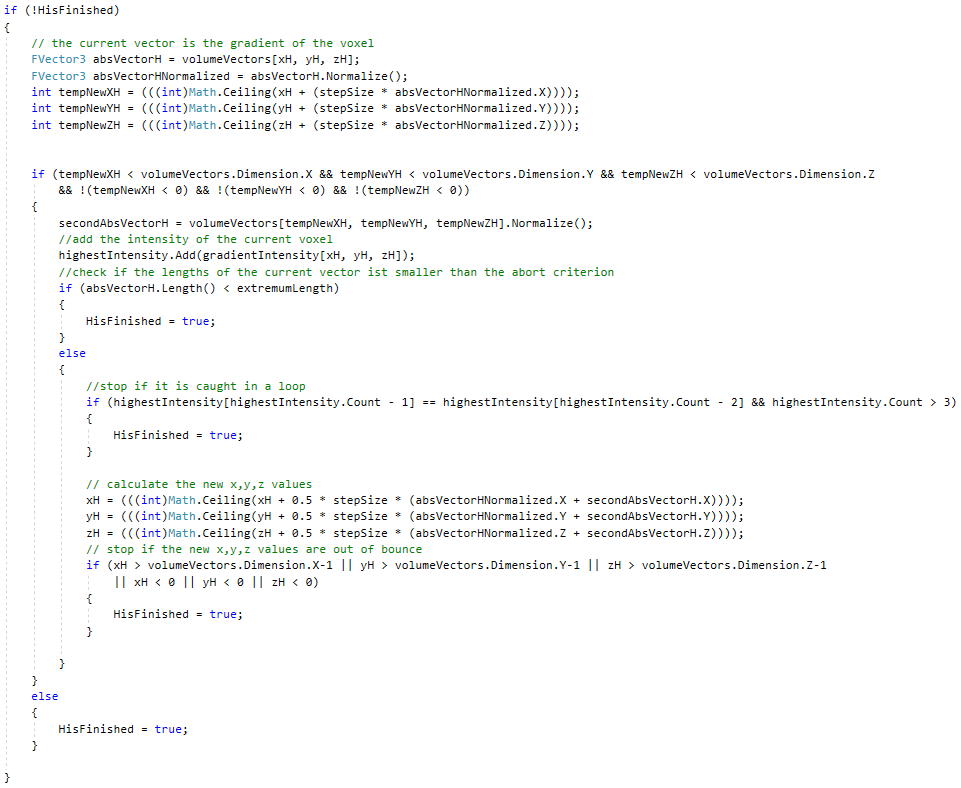
\includegraphics[width=1.2\textwidth]{Logos/LH_Code.PNG}
\caption{Implementierung der Berechnung der High-Werte} 
\label{fig:lh_code} 
\end{figure}


In \autoref{fig:lh_code} kann man den Code zur Berechnung eines High-Wertes sehen. Der Code liegt innerhalb einer while-Schleife, die so lange aufgerufen wird, bis \textit{HisFinished} und \textit{LisFinished} true sind. Die Berechnung des Low-Wertes ist ebenfalls in der Schleife und sieht bis auf die Richtung der neuen \textit{absVector} und \textit{secondAbsVector} gleich aus.
\newline
Am Anfang eines Durchlaufes wird der normalisierte Gradienten des aktuellen Punktes in \textit{absVectorNormalized} gespeichert. Anschließend wird der Punkt des zweiten normalisierten Vektors berechnet. Liegt dieser außerhalb des Volumens, so wird die Integration beendet. und der Wert des letzten besuchten Voxels als Ergebnis zurückgegeben, da das Ergebnis immer der letzte Eintrag der Liste \textit{highestIntensity} ist. Liegt er jedoch innerhalb des Volumens, so wird der \textit{secondAbsVector} berechnet und der Intensitätswert des aktuellen Punktes zu der Liste hinzugefügt. Ist der Gradient des aktuellen Punktes kleiner als \textit{extremumLength}, was im Falle von CT-Daten bei null liegt, wird die Integration beendet. Andernfalls wird der neue Punkt mithilfe von \textit{absVectorNormalized} und \textit{secondAbsVecotr} gemäß Hong's Verfahren \cite{} ermittelt. Erneut endet die Integration, falls dieser Punkt außerhalb des Volumens liegt. Vor der Berechnung des nächsten Punktes, wird jedoch über die \textit{highestIntensity} Liste nach Schleifen gesucht. Bei sehr kleinen Gradienten, die jedoch größer als null sind, kann es vorkommen, dass das Verfahren immer wieder den selben Punkt findet und somit in einer Endlosschleife feststeckt. Diese Kontrolle könnte jedoch über die Koordinaten der iterierten Punkte geschehen, um dem unwahrscheinlichem Fall, dass zwei durch die Integration hintereinander gefundenen Punkte genau den selben Intensitätswert haben.
\newline
Dieser Vorgang wiederholt sich für den High- als auch für den Low-Wert solange, bis die Integration aus einem der gegebenen Abbruchkriterien stoppt.